
\subsection{Kinematik}

\subsubsection{Aufgaben}
Die Kinematik dient als Grundstein für die Pfadberechnung erfüllt zwei elementare Aufgaben. Mit Hilfe der direkten Kinematik kann, bei gegebenen Winkelstellungen und Achsenlängen, die aktuelle Position des Werkzeugs im Koordinatensystem berechnet werden. Für die Interpolation von wesentlich größerer Bedeutung, ist jedoch die inverse Kinematik mit welcher die Winkelstellungen der Achsen, bei gegebenen Zielpunkt und Achsenlängen, berechnet werden können.

\subsubsection{Aufbau}
Die Verfahren zur direkten beziehungsweise indirekten Kinematik sind in der Klasse Kinematics als statische Methoden \textit{CalculateDirect} und \textit{CalculateInverse} implementiert.

\subsubsection{Umsetzung}

\textbf{Kinematics}\\
Die im Aufbau erwähnten Methoden der Kinematics-Klasse sind wie folgt implementiert:
\begin{itemize}
\item \textbf{CalculateDirect}\\
Bei Aufruf dieser Methode wird mit dem Verfahren der direkten Kinematik und den angegebenen Parametern die Position des Werkzeugs, bei gegebenen Winkelstellungen und Achsenlängen berechnet. Als Parameter werden ihr die Winkelstellungen der ersten Achse $\alpha_1$ und der zweiten Achse $\alpha_2$, die Länge der ersten und zweiten Achse, $l_1$ und $l_2$, sowie die Werkzeugreichweite $d_w$ und die Übersetzung der transversalen Achse $\omega$ als \textit{float}-Werte übergeben. Mit diesen Informationen kann nun berechnet werden an welchem Punkt sich das Werkzeug im Koordinatensystem befindet.
\begin{figure}[H]
  \centering
  \begin{minipage}[t]{12 cm}
  	\centering
  	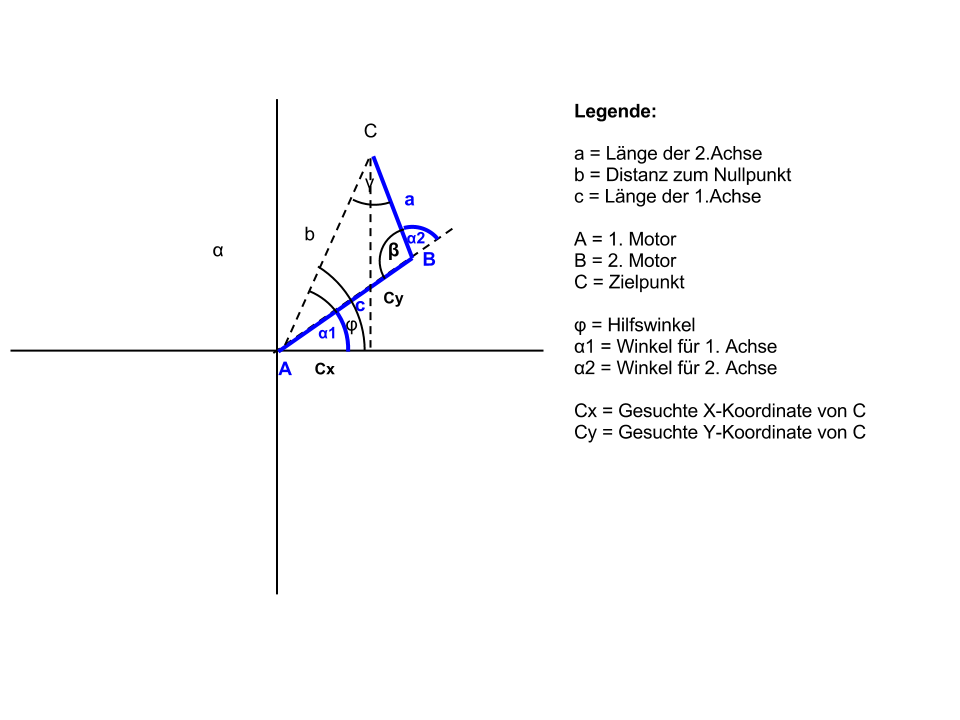
\includegraphics[width=12cm]{images/Direktkinematik} 
    \caption{Skizze zur direkten Kinematik}
  \end{minipage}
\end{figure}
\newpage
Der Punkt wird nach folgendem Schema berechnet:
\begin{enumerate}
\item Berechnung des Winkels $\beta$\\
Der Winkel $\beta$ kann bei gegebenenen $\alpha_2$ relativ einfach berechnet werden (siehe Skizze) und ist nötig um anschließend die Distanz $d$ zu berechnen. Es wird der Betrag von $\alpha_2$ verwendet, da dieser Winkel je nach Achskonfiguration negativ sein kann.
\begin{align*}
\beta = 180^\circ - |\alpha_2|
\end{align*}
\item Berechnung der Distanz $d$\\
Um $d$ zu berechnen wird der Kosinussatz für $\beta$ verwendet:
\begin{align*}
b^2 = a^2+c^2-2ac\cos\beta \\
b = \sqrt{a^2+c^2-2ac\cos\beta}
\end{align*}
Angepasst an unsere Variablen entsteht daraus die Formel:
\begin{align*}
d = \sqrt{l_1^2+l_2^2-2l_1l_2\cos\beta}
\end{align*}
\item Berechnung des Winkels $\alpha$\\
Um zu den gesuchten Koordinaten zu gelangen benötigen wir den Referenzwinkel $\varphi$, welcher aus der Summe von $\alpha$ und $\alpha1$ definiert ist. Der Winkel $\alpha$ kann über die Umformung des Kosinussatzes berechnet werden:
\begin{align*}
a^2 & = b^2 + c^2 - 2bc \cos \alpha \\
2bc \cos \alpha & = b^2 + c^2 - a^2 \\
\cos \alpha & = \frac{b^2 + c^2 - a^2}{2bc} \\
\alpha & = \arccos \frac{b^2 + c^2 - a^2}{2bc}
\end{align*}
Angepasst an unsere Variablen entsteht daraus die Formel:
\begin{align*}
\alpha = \arccos \frac{d^2 + l_1^2 - l_2^2}{2dl_1}
\end{align*}
\newpage
\item Berechnung des Referenzwinkels $\varphi$\\
Über den Winkel $\alpha_2$ kann auf die Achskonfiguration geschlossen werden.
Bei Achskonfiguration "'Lefty"':
\begin{align*}
\varphi = \alpha_1 + \alpha
\end{align*}
Bei Achskonfiguration "'Righty"':
\begin{align*}
\varphi = \alpha_1 - \alpha
\end{align*}
\item Berechnung des gesuchten Punkts\\
Mit dem nun vorhandenen Zahlenmaterial kann nun der gesuchte Punkte über die Sinus beziehungsweise Kosinus-Funktion im rechtwinkeligen Dreieck berechnet werden.\\
Die z-Koordinate kann über $\alpha3$, die Übersetzung $\omega$ und die Werkzeugreichweite $d_w$ hergeleitet werden.
\begin{align*}
x &= d * \cos \varphi \\
y &= d * \sin \varphi \\
z &= d_w - (\frac{\alpha3}{\omega})
\end{align*}
\end{enumerate}
\newpage
\item \textbf{CalculateInverse}\\
Bei Aufruf dieser Methode wird mit dem Verfahren der inversen Kinematik und den angegebenen Parametern eine Menge an möglichen Winkelstellungen der Achsen am angegeben Zielpunkt berechnet. Als Parameter werden ihr der Zielpunkt als \textit{Point3D}-Objekt, die Länge der ersten und zweiten Achse, $l_1$ und $l_2$, sowie die Werkzeugreichweite $d_w$ und die Übersetzung der transversalen Achse $\omega$ als \textit{float}-Werte übergeben.\\
Aus diesen Informationen berechnet die Methode die möglichen Gelenkstellungen und gibt diese in Form eines \textit{InterpolationStep}-Arrays zurück.
\begin{figure}[H]
  \centering
  \begin{minipage}[t]{12 cm}
  	\centering
  	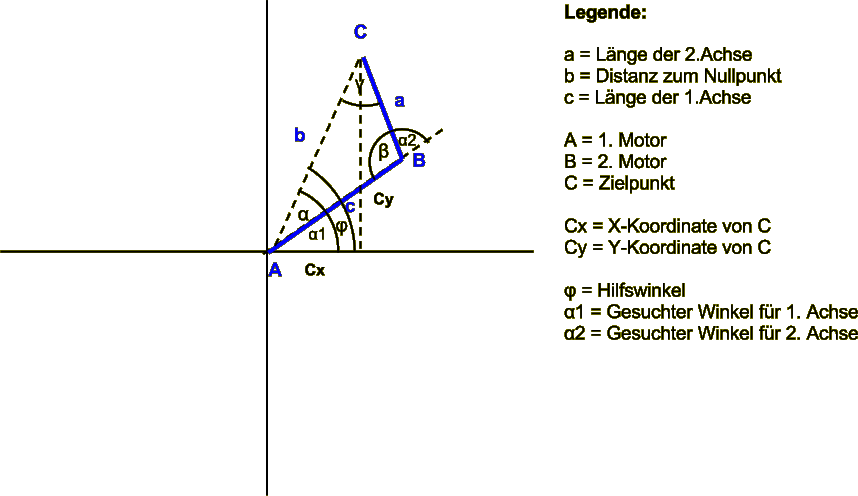
\includegraphics[width=12cm]{images/Inverskinematik} 
    \caption{Skizze zur inversen Kinematik}
  \end{minipage}
\end{figure}
Die Berechnung der möglichen Gelenkstellungen läuft nach folgendem Schema ab:
\begin{enumerate}
\item Deklarieren der Hilfsvariablen\\
Zur Vereinfachung der Berechnung werden zuerst die Variablen $x$,$y$,$z$ vom Typ \textit{float} definiert. Diesen Variablen werden entsprechend die X-,Y- und Z-Koordinaten des Zielpunkts zugewiesen.
\item Berechnung der Distanz $d$\\
Zur Berechnung der Winkel werden die Seitenlängen des allgemeinen Dreiecks, welches durch die beiden Achsen $l_1$ und $l_2$ sowie die Distanz zum Zielpunkt $d$ gebildet wird, benötigt. Da die Längen der Achsen bereits bekannt sind, muss nur die Distanz d durch Verwendung des Satzes des Pythagoras zusammen mit den x- und y-Koordinaten berechnet werden.\\
\begin{equation*}
d = \sqrt{x^2 + y^2}
\end{equation*}
\newpage
\item Berechnung der Innenwinkel\\
Da nun alle drei Seitenlängen bekannt sind, können die Innenwinkel $\alpha$, $\beta$, $\gamma$ über den Kosinussatz berechnet werden.\\
\\
Umformung des Kosinussatzes für $\alpha$:
\begin{align*}
a^2 & = b^2 + c^2 - 2bc \cos \alpha \\
2bc \cos \alpha & = b^2 + c^2 - a^2 \\
\cos \alpha & = \frac{b^2 + c^2 - a^2}{2bc} \\
\alpha & = \arccos \frac{b^2 + c^2 - a^2}{2bc}
\end{align*}
Umformung des Kosinussatzes für $\beta$:
\begin{align*}
b^2 & = a^2 + c^2 - 2ac \cos \beta \\
2ac \cos \beta & = a^2 + c^2 - b^2 \\
\cos \beta & = \frac{a^2 + c^2 - b^2}{2ac} \\
\beta & = \arccos \frac{a^2 + c^2 - b^2}{2ac}
\end{align*}
Umformung des Kosinussatzes für $\gamma$:
\begin{align*}
c^2 = a^2 + b^2 - 2ab \cos \gamma \\
2ab \cos \gamma = a^2 + b^2 - c^2 \\
\cos \gamma = \frac{a^2 + b^2 - c^2}{2ab} \\
\gamma = \arccos \frac{a^2 + b^2 - c^2}{2ab}
\end{align*}
Auf unsere Variablen angepasst sehen die Formeln für die Berechnung der Winkel folgendermaßen aus:
\begin{align*}
\alpha = \arccos \frac{d^2 + l_1^2 - l_2^2}{2dl_1} \\
\beta = \arccos \frac{l_2^2 + l_1^2 - d^2}{2l_1l_2} \\
\gamma = \arccos \frac{d^2 + l_2^2 - l_1^2}{2dl_2}
\end{align*}
\newpage
\item Berechnung des Referenzwinkels $\varphi$:\\
Im nächsten Schritt wird noch der Referenzwinkel $\varphi$, welcher die Position des Dreiecks im Koordinatensystem festlegt, berechnet. Dieser Winkel befindet sich in einem rechtwinkeligen Dreieck, welches durch $d$, $x$ und $y$ definiert wird und kann durch Umformung der Sinusfunktion im rechtwinkeligen Dreieck berechnet werden:
\begin{align*}
\varphi = \arccos \frac{x}{d}
\end{align*}
\item Überprüfen des Quadranten:\\
Da die Arkussinus-Funktion lediglich einen Winkel zwischen 0$^\circ$ und 180$^\circ$ liefert, muss der Quadrant in dem sich der Zielpunkt befindet überprüft werden. Befindet sich dieser im 3. oder 4. Quadranten, so wird das Vorzeichen des Referenzwinkels $\varphi$ umgedreht. 
\item Berechnung von $\alpha_1$,$\alpha_2$ und $\alpha3$\\
Mit dem nun vorhandenen Zahlenmaterial können die gesuchten Winkel der ersten und zweiten Achse folgendermaßen berechnet werden:
\begin{itemize}
\item Berechnung von $\alpha_1$:\\
Die möglichen Winkel der ersten Achse ergeben sich aus der Differenz beziehungsweise Summe des Referenzwinkels $\varphi$ und des Innenwinkels $\alpha$
\begin{align*}
1. Gelenkstellung: \alpha_1 &= \varphi - \alpha \\
2. Gelenkstellung: \alpha_1 &= \varphi + \alpha
\end{align*}
\item Berechnung von $\alpha_2$:\\
Der möglichen Winkel der zweiten Achse ergeben sich aus der Differenz zwischen 180$^\circ$ und dem Innenwinkel $\beta$
\begin{align*}
1. Gelenkstellung: \alpha_2 = 180 - \beta \\
2. Gelenkstellung: \alpha_2 = \beta - 180
\end{align*}
\item Berechnung von $\alpha_3$:\\
Da die Position der transversalen Achse ein Zusammenspiel aus der Winkelstellung des entsprechenden Motors, der Reichweite des Werkzeugs $d_w$ und der Übersetzung $\omega$ ist gibt es nur eine einzige Lösung.
\begin{align*}
\alpha_3 = (d_w-z)\omega
\end{align*}
\end{itemize}

\end{enumerate}
Aus den berechneten Werten, werden zwei \textit{InterpolationStep}-Objekt erzeugt, welche die möglichen Gelenkstellungen an diesem Punkt enthalten. Letztere werden als \textit{InterpolationStep}-Array zurückgegeben, wobei sich die 1.Gelenkstellung am Index 0 und die 2.Gelenkstellung am Index 1 befindet.
\end{itemize}

\textbf{AxisConfiguration}\\
Diese Enumeration definiert zwei Konfigurationen, welche bei der Auswahl der, von der Inverskinematik berechneten, zum Einsatz kommen. Jeder Adapter enthält ein Property \textit{AxisConfiguration}, welche die aktuelle Konfiguration des Adapters festlegt. Kann ein Punkt im Koordinatensystem mit der aktuellen Konfiguration nicht erreicht werden, so kann diese mit einem \textit{ChangeConfigurationCommand} geändert werden.
Bei dem, in dieser Diplomarbeit angenommenen, Robotermodell gibt es zwei Konfigurationsmöglichkeiten:
\begin{itemize}
\item \textbf{Lefty}\\
Die zweite Achse ist immer nach links gerichtet, daher der Winkel $\alpha_2$ in diesem Fall immer positiv.
\item \textbf{Righty}\\
Die zweite Achse ist immer nach rechts gerichtet, daher der Winkel $\alpha_2$ in diesem Fall immer negativ.
\end{itemize}

\begin{figure}[H]
  \centering
  \begin{minipage}[t]{12 cm}
  	\centering
  	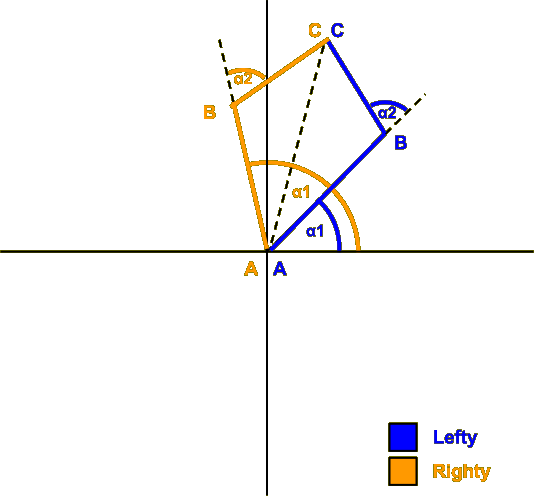
\includegraphics[width=8cm]{images/AxisConfiguration} 
    \caption{Darstellung der Achskonfigurationen}
  \end{minipage}
\end{figure}
